%% LyX 2.1.4 created this file.  For more info, see http://www.lyx.org/.
%% Do not edit unless you really know what you are doing.
\documentclass[american,fontsize=11pt,paper=a4,twoside,openright,titlepage,numbers=noenddot,headinclude,BCOR=5mm,footinclude=true,cleardoublepage=empty]{scrreprt}
\usepackage[T1]{fontenc}
\usepackage[utf8]{inputenc}
\setcounter{secnumdepth}{2}
\usepackage{color}
\usepackage{array}
\usepackage{verbatim}
\usepackage{booktabs}
\usepackage{amsmath}
\usepackage{amssymb}
\usepackage{graphicx}

\makeatletter

%%%%%%%%%%%%%%%%%%%%%%%%%%%%%% LyX specific LaTeX commands.
%% Because html converters don't know tabularnewline
\providecommand{\tabularnewline}{\\}

%%%%%%%%%%%%%%%%%%%%%%%%%%%%%% Textclass specific LaTeX commands.
% Classic Thesis Style loader
\makeatother
% ****************************************************************************************************
% classicthesis-config.tex 
% formerly known as loadpackages.sty, classicthesis-ldpkg.sty, and classicthesis-preamble.sty 
% Use it at the beginning of your ClassicThesis.tex, or as a LaTeX Preamble 
% in your ClassicThesis.{tex,lyx} with % ****************************************************************************************************
% classicthesis-config.tex 
% formerly known as loadpackages.sty, classicthesis-ldpkg.sty, and classicthesis-preamble.sty 
% Use it at the beginning of your ClassicThesis.tex, or as a LaTeX Preamble 
% in your ClassicThesis.{tex,lyx} with % ****************************************************************************************************
% classicthesis-config.tex 
% formerly known as loadpackages.sty, classicthesis-ldpkg.sty, and classicthesis-preamble.sty 
% Use it at the beginning of your ClassicThesis.tex, or as a LaTeX Preamble 
% in your ClassicThesis.{tex,lyx} with \input{classicthesis-config}
% ****************************************************************************************************  
% If you like the classicthesis, then I would appreciate a postcard. 
% My address can be found in the file ClassicThesis.pdf. A collection 
% of the postcards I received so far is available online at 
% http://postcards.miede.de
% ****************************************************************************************************


% ****************************************************************************************************
% 0. Set the encoding of your files. UTF-8 is the only sensible encoding nowadays. If you can't read
% äöüßáéçèê∂åëæƒÏ€ then change the encoding setting in your editor, not the line below. If your editor
% does not support utf8 use another editor!
% ****************************************************************************************************
\PassOptionsToPackage{utf8}{inputenc}
	\usepackage{inputenc}

% ****************************************************************************************************
% 1. Configure classicthesis for your needs here, e.g., remove "drafting" below 
% in order to deactivate the time-stamp on the pages
% ****************************************************************************************************
\PassOptionsToPackage{eulerchapternumbers,listings,drafting,%
					 pdfspacing,floatperchapter,%linedheaders,%
					 subfig,beramono,parts}{classicthesis}                                        
% ********************************************************************
% Available options for classicthesis.sty 
% (see ClassicThesis.pdf for more information):
% drafting
% parts nochapters linedheaders
% eulerchapternumbers beramono eulermath pdfspacing minionprospacing
% tocaligned dottedtoc manychapters
% listings floatperchapter subfig
% ********************************************************************


% ****************************************************************************************************
% 2. Personal data and user ad-hoc commands
% ****************************************************************************************************
\newcommand{\myTitle}{Molecular Density Functional Theory\xspace}
\newcommand{\mytitle}{under homogeneous reference fluid approximation\xspace}
\newcommand{\mySubtitle}{Systematic prediction of solvation properties\xspace}
\newcommand{\mysubtitle}{with molecular-scale liquid theory\xspace}
\newcommand{\myDegree}{\xspace}
\newcommand{\myName}{Lu Ding\xspace}
\newcommand{\myProf}{Daniel Borgis, Luc Belloni\xspace}
\newcommand{\myOtherProf}{Maximilien Levesque\xspace}
\newcommand{\mySupervisor}{Put name here\xspace}
\newcommand{\myFaculty}{Put data here\xspace}
\newcommand{\myDepartment}{Put data here\xspace}
\newcommand{\myUni}{Put data here\xspace}
\newcommand{\myLocation}{Maison de la Simulation, CEA Saclay\xspace}
\newcommand{\myTime}{21 September 2016\xspace}
\newcommand{\myVersion}{version 3.3}

% ********************************************************************
% Setup, finetuning, and useful commands
% ********************************************************************
\newcounter{dummy} % necessary for correct hyperlinks (to index, bib, etc.)
\newlength{\abcd} % for ab..z string length calculation
\providecommand{\mLyX}{L\kern-.1667em\lower.25em\hbox{Y}\kern-.125emX\@}
\newcommand{\ie}{i.\,e.}
\newcommand{\Ie}{I.\,e.}
\newcommand{\eg}{e.\,g.}
\newcommand{\Eg}{E.\,g.} 
% ****************************************************************************************************


% ****************************************************************************************************
% 3. Loading some handy packages
% ****************************************************************************************************
% ******************************************************************** 
% Packages with options that might require adjustments
% ******************************************************************** 
%\PassOptionsToPackage{ngerman,american}{babel}   % change this to your language(s)
% Spanish languages need extra options in order to work with this template
%\PassOptionsToPackage{spanish,es-lcroman}{babel}
	\usepackage{babel}

\usepackage{csquotes}
\PassOptionsToPackage{%
    %backend=biber, %instead of bibtex
    backend=bibtex8,%bibencoding=ascii,%
    language=auto,%
    style=numeric-comp,%
    %style=philosophy-modern,%
    %style=authoryear-comp, % Author 1999, 2010
    %bibstyle=authoryear,dashed=false, % dashed: substitute rep. author with ---
    sorting=nyt, % name, year, title
    maxbibnames=10, % default: 3, et al.
    %backref=true,%
    natbib=true % natbib compatibility mode (\citep and \citet still work)
}{biblatex}
    \usepackage{biblatex}

\PassOptionsToPackage{fleqn}{amsmath}       % math environments and more by the AMS 
    \usepackage{amsmath}

% ******************************************************************** 
% General useful packages
% ******************************************************************** 
\PassOptionsToPackage{T1}{fontenc} % T2A for cyrillics
    \usepackage{fontenc}     
\usepackage{textcomp} % fix warning with missing font shapes
\usepackage{scrhack} % fix warnings when using KOMA with listings package          
\usepackage{xspace} % to get the spacing after macros right  
\usepackage{mparhack} % get marginpar right
\usepackage{fixltx2e} % fixes some LaTeX stuff --> since 2015 in the LaTeX kernel (see below)
%\usepackage[latest]{latexrelease} % will be used once available in more distributions (ISSUE #107)
\PassOptionsToPackage{printonlyused,smaller}{acronym}
    \usepackage{acronym} % nice macros for handling all acronyms in the thesis
   %\renewcommand{\bflabel}[1]{{#1}\hfill} % fix the list of acronyms --> no longer working
   %\renewcommand*{\aclabelfont}[1]{\spacedlowsmallcaps{#1}}
    \renewcommand*{\acsfont}[1]{{\rmfamily\mdseries\small#1}} 
% ****************************************************************************************************


% ****************************************************************************************************
% 4. Setup floats: tables, (sub)figures, and captions
% ****************************************************************************************************
\usepackage{tabularx} % better tables
    \setlength{\extrarowheight}{3pt} % increase table row height
\newcommand{\tableheadline}[1]{\multicolumn{1}{c}{\spacedlowsmallcaps{#1}}}
\newcommand{\myfloatalign}{\centering} % to be used with each float for alignment
\usepackage{caption}
% Thanks to cgnieder and Claus Lahiri
% http://tex.stackexchange.com/questions/69349/spacedlowsmallcaps-in-caption-label
% [REMOVED DUE TO OTHER PROBLEMS, SEE ISSUE #82]    
%\DeclareCaptionLabelFormat{smallcaps}{\bothIfFirst{#1}{~}\MakeTextLowercase{\textsc{#2}}}
%\captionsetup{font=small,labelformat=smallcaps} % format=hang,
\captionsetup{font=small} % format=hang,
\usepackage{subfig}  
% ****************************************************************************************************


% ****************************************************************************************************
% 5. Setup code listings
% ****************************************************************************************************
\usepackage{listings} 
%\lstset{emph={trueIndex,root},emphstyle=\color{BlueViolet}}%\underbar} % for special keywords
\lstset{language=[LaTeX]Tex,%C++,
    keywordstyle=\color{RoyalBlue},%\bfseries,
    basicstyle=\small\ttfamily,
    %identifierstyle=\color{NavyBlue},
    commentstyle=\color{Green}\ttfamily,
    stringstyle=\rmfamily,
    numbers=none,%left,%
    numberstyle=\scriptsize,%\tiny
    stepnumber=5,
    numbersep=8pt,
    showstringspaces=false,
    breaklines=true,
    frameround=ftff,
    frame=single,
    belowcaptionskip=.75\baselineskip
    %frame=L
} 
% ****************************************************************************************************             


% ****************************************************************************************************
% 6. PDFLaTeX, hyperreferences and citation backreferences
% ****************************************************************************************************
% ********************************************************************
% Using PDFLaTeX
% ********************************************************************
\PassOptionsToPackage{pdftex,hyperfootnotes=false,pdfpagelabels}{hyperref}
    \usepackage{hyperref}  % backref linktocpage pagebackref
\pdfcompresslevel=9
\pdfadjustspacing=1 
\PassOptionsToPackage{pdftex}{graphicx}
    \usepackage{graphicx} 
 

% ********************************************************************
% Hyperreferences
% ********************************************************************
\hypersetup{%
    %draft, % = no hyperlinking at all (useful in b/w printouts)
    colorlinks=false, linktocpage=true, pdfstartpage=3, pdfstartview=FitV,%
    % uncomment the following line if you want to have black links (e.g., for printing)
    %colorlinks=false, linktocpage=false, pdfstartpage=3, pdfstartview=FitV, pdfborder={0 0 0},%
    breaklinks=true, pdfpagemode=UseNone, pageanchor=true, pdfpagemode=UseOutlines,%
    plainpages=false, bookmarksnumbered, bookmarksopen=true, bookmarksopenlevel=1,%
    hypertexnames=true, pdfhighlight=/O,%nesting=true,%frenchlinks,%
    urlcolor=webbrown, linkcolor=RoyalBlue, citecolor=webgreen, %pagecolor=RoyalBlue,%
    %urlcolor=Black, linkcolor=Black, citecolor=Black, %pagecolor=Black,%
    pdftitle={\myTitle},%
    pdfauthor={\textcopyright\ \myName, \myUni, \myFaculty},%
    pdfsubject={},%
    pdfkeywords={},%
    pdfcreator={pdfLaTeX},%
    pdfproducer={LaTeX with hyperref and classicthesis}%
}   

% ********************************************************************
% Setup autoreferences
% ********************************************************************
% There are some issues regarding autorefnames
% http://www.ureader.de/msg/136221647.aspx
% http://www.tex.ac.uk/cgi-bin/texfaq2html?label=latexwords
% you have to redefine the makros for the 
% language you use, e.g., american, ngerman
% (as chosen when loading babel/AtBeginDocument)
% ********************************************************************
\makeatletter
\@ifpackageloaded{babel}%
    {%
       \addto\extrasamerican{%
			\renewcommand*{\figureautorefname}{Figure}%
			\renewcommand*{\tableautorefname}{Table}%
			\renewcommand*{\partautorefname}{Part}%
			\renewcommand*{\chapterautorefname}{Chapter}%
			\renewcommand*{\sectionautorefname}{Section}%
			\renewcommand*{\subsectionautorefname}{Section}%
			\renewcommand*{\subsubsectionautorefname}{Section}%     
                }%
       \addto\extrasngerman{% 
			\renewcommand*{\paragraphautorefname}{Absatz}%
			\renewcommand*{\subparagraphautorefname}{Unterabsatz}%
			\renewcommand*{\footnoteautorefname}{Fu\"snote}%
			\renewcommand*{\FancyVerbLineautorefname}{Zeile}%
			\renewcommand*{\theoremautorefname}{Theorem}%
			\renewcommand*{\appendixautorefname}{Anhang}%
			\renewcommand*{\equationautorefname}{Gleichung}%        
			\renewcommand*{\itemautorefname}{Punkt}%
                }%  
            % Fix to getting autorefs for subfigures right (thanks to Belinda Vogt for changing the definition)
            \providecommand{\subfigureautorefname}{\figureautorefname}%             
    }{\relax}
\makeatother


% ****************************************************************************************************
% 7. Last calls before the bar closes
% ****************************************************************************************************
% ********************************************************************
% Development Stuff
% ********************************************************************
\listfiles
%\PassOptionsToPackage{l2tabu,orthodox,abort}{nag}
%   \usepackage{nag}
%\PassOptionsToPackage{warning, all}{onlyamsmath}
%   \usepackage{onlyamsmath}

% ********************************************************************
% Last, but not least...
% ********************************************************************
\usepackage{classicthesis} 
\usepackage{lmodern}
% ****************************************************************************************************


% ****************************************************************************************************
% 8. Further adjustments (experimental)
% ****************************************************************************************************
% ********************************************************************
% Changing the text area
% ********************************************************************
%\linespread{1.05} % a bit more for Palatino
%\areaset[current]{312pt}{761pt} % 686 (factor 2.2) + 33 head + 42 head \the\footskip
%\setlength{\marginparwidth}{7em}%
%\setlength{\marginparsep}{2em}%

% ********************************************************************
% Using different fonts
% ********************************************************************
%\usepackage[oldstylenums]{kpfonts} % oldstyle notextcomp
%\usepackage[osf]{libertine}
%\usepackage[light,condensed,math]{iwona}
%\renewcommand{\sfdefault}{iwona}
%\usepackage{lmodern} % <-- no osf support :-(
%\usepackage{cfr-lm} % 
%\usepackage[urw-garamond]{mathdesign} <-- no osf support :-(
%\usepackage[default,osfigures]{opensans} % scale=0.95 
%\usepackage[sfdefault]{FiraSans}
% ****************************************************************************************************

% ****************************************************************************************************  
% If you like the classicthesis, then I would appreciate a postcard. 
% My address can be found in the file ClassicThesis.pdf. A collection 
% of the postcards I received so far is available online at 
% http://postcards.miede.de
% ****************************************************************************************************


% ****************************************************************************************************
% 0. Set the encoding of your files. UTF-8 is the only sensible encoding nowadays. If you can't read
% äöüßáéçèê∂åëæƒÏ€ then change the encoding setting in your editor, not the line below. If your editor
% does not support utf8 use another editor!
% ****************************************************************************************************
\PassOptionsToPackage{utf8}{inputenc}
	\usepackage{inputenc}

% ****************************************************************************************************
% 1. Configure classicthesis for your needs here, e.g., remove "drafting" below 
% in order to deactivate the time-stamp on the pages
% ****************************************************************************************************
\PassOptionsToPackage{eulerchapternumbers,listings,drafting,%
					 pdfspacing,floatperchapter,%linedheaders,%
					 subfig,beramono,parts}{classicthesis}                                        
% ********************************************************************
% Available options for classicthesis.sty 
% (see ClassicThesis.pdf for more information):
% drafting
% parts nochapters linedheaders
% eulerchapternumbers beramono eulermath pdfspacing minionprospacing
% tocaligned dottedtoc manychapters
% listings floatperchapter subfig
% ********************************************************************


% ****************************************************************************************************
% 2. Personal data and user ad-hoc commands
% ****************************************************************************************************
\newcommand{\myTitle}{Molecular Density Functional Theory\xspace}
\newcommand{\mytitle}{under homogeneous reference fluid approximation\xspace}
\newcommand{\mySubtitle}{Systematic prediction of solvation properties\xspace}
\newcommand{\mysubtitle}{with molecular-scale liquid theory\xspace}
\newcommand{\myDegree}{\xspace}
\newcommand{\myName}{Lu Ding\xspace}
\newcommand{\myProf}{Daniel Borgis, Luc Belloni\xspace}
\newcommand{\myOtherProf}{Maximilien Levesque\xspace}
\newcommand{\mySupervisor}{Put name here\xspace}
\newcommand{\myFaculty}{Put data here\xspace}
\newcommand{\myDepartment}{Put data here\xspace}
\newcommand{\myUni}{Put data here\xspace}
\newcommand{\myLocation}{Maison de la Simulation, CEA Saclay\xspace}
\newcommand{\myTime}{21 September 2016\xspace}
\newcommand{\myVersion}{version 3.3}

% ********************************************************************
% Setup, finetuning, and useful commands
% ********************************************************************
\newcounter{dummy} % necessary for correct hyperlinks (to index, bib, etc.)
\newlength{\abcd} % for ab..z string length calculation
\providecommand{\mLyX}{L\kern-.1667em\lower.25em\hbox{Y}\kern-.125emX\@}
\newcommand{\ie}{i.\,e.}
\newcommand{\Ie}{I.\,e.}
\newcommand{\eg}{e.\,g.}
\newcommand{\Eg}{E.\,g.} 
% ****************************************************************************************************


% ****************************************************************************************************
% 3. Loading some handy packages
% ****************************************************************************************************
% ******************************************************************** 
% Packages with options that might require adjustments
% ******************************************************************** 
%\PassOptionsToPackage{ngerman,american}{babel}   % change this to your language(s)
% Spanish languages need extra options in order to work with this template
%\PassOptionsToPackage{spanish,es-lcroman}{babel}
	\usepackage{babel}

\usepackage{csquotes}
\PassOptionsToPackage{%
    %backend=biber, %instead of bibtex
    backend=bibtex8,%bibencoding=ascii,%
    language=auto,%
    style=numeric-comp,%
    %style=philosophy-modern,%
    %style=authoryear-comp, % Author 1999, 2010
    %bibstyle=authoryear,dashed=false, % dashed: substitute rep. author with ---
    sorting=nyt, % name, year, title
    maxbibnames=10, % default: 3, et al.
    %backref=true,%
    natbib=true % natbib compatibility mode (\citep and \citet still work)
}{biblatex}
    \usepackage{biblatex}

\PassOptionsToPackage{fleqn}{amsmath}       % math environments and more by the AMS 
    \usepackage{amsmath}

% ******************************************************************** 
% General useful packages
% ******************************************************************** 
\PassOptionsToPackage{T1}{fontenc} % T2A for cyrillics
    \usepackage{fontenc}     
\usepackage{textcomp} % fix warning with missing font shapes
\usepackage{scrhack} % fix warnings when using KOMA with listings package          
\usepackage{xspace} % to get the spacing after macros right  
\usepackage{mparhack} % get marginpar right
\usepackage{fixltx2e} % fixes some LaTeX stuff --> since 2015 in the LaTeX kernel (see below)
%\usepackage[latest]{latexrelease} % will be used once available in more distributions (ISSUE #107)
\PassOptionsToPackage{printonlyused,smaller}{acronym}
    \usepackage{acronym} % nice macros for handling all acronyms in the thesis
   %\renewcommand{\bflabel}[1]{{#1}\hfill} % fix the list of acronyms --> no longer working
   %\renewcommand*{\aclabelfont}[1]{\spacedlowsmallcaps{#1}}
    \renewcommand*{\acsfont}[1]{{\rmfamily\mdseries\small#1}} 
% ****************************************************************************************************


% ****************************************************************************************************
% 4. Setup floats: tables, (sub)figures, and captions
% ****************************************************************************************************
\usepackage{tabularx} % better tables
    \setlength{\extrarowheight}{3pt} % increase table row height
\newcommand{\tableheadline}[1]{\multicolumn{1}{c}{\spacedlowsmallcaps{#1}}}
\newcommand{\myfloatalign}{\centering} % to be used with each float for alignment
\usepackage{caption}
% Thanks to cgnieder and Claus Lahiri
% http://tex.stackexchange.com/questions/69349/spacedlowsmallcaps-in-caption-label
% [REMOVED DUE TO OTHER PROBLEMS, SEE ISSUE #82]    
%\DeclareCaptionLabelFormat{smallcaps}{\bothIfFirst{#1}{~}\MakeTextLowercase{\textsc{#2}}}
%\captionsetup{font=small,labelformat=smallcaps} % format=hang,
\captionsetup{font=small} % format=hang,
\usepackage{subfig}  
% ****************************************************************************************************


% ****************************************************************************************************
% 5. Setup code listings
% ****************************************************************************************************
\usepackage{listings} 
%\lstset{emph={trueIndex,root},emphstyle=\color{BlueViolet}}%\underbar} % for special keywords
\lstset{language=[LaTeX]Tex,%C++,
    keywordstyle=\color{RoyalBlue},%\bfseries,
    basicstyle=\small\ttfamily,
    %identifierstyle=\color{NavyBlue},
    commentstyle=\color{Green}\ttfamily,
    stringstyle=\rmfamily,
    numbers=none,%left,%
    numberstyle=\scriptsize,%\tiny
    stepnumber=5,
    numbersep=8pt,
    showstringspaces=false,
    breaklines=true,
    frameround=ftff,
    frame=single,
    belowcaptionskip=.75\baselineskip
    %frame=L
} 
% ****************************************************************************************************             


% ****************************************************************************************************
% 6. PDFLaTeX, hyperreferences and citation backreferences
% ****************************************************************************************************
% ********************************************************************
% Using PDFLaTeX
% ********************************************************************
\PassOptionsToPackage{pdftex,hyperfootnotes=false,pdfpagelabels}{hyperref}
    \usepackage{hyperref}  % backref linktocpage pagebackref
\pdfcompresslevel=9
\pdfadjustspacing=1 
\PassOptionsToPackage{pdftex}{graphicx}
    \usepackage{graphicx} 
 

% ********************************************************************
% Hyperreferences
% ********************************************************************
\hypersetup{%
    %draft, % = no hyperlinking at all (useful in b/w printouts)
    colorlinks=false, linktocpage=true, pdfstartpage=3, pdfstartview=FitV,%
    % uncomment the following line if you want to have black links (e.g., for printing)
    %colorlinks=false, linktocpage=false, pdfstartpage=3, pdfstartview=FitV, pdfborder={0 0 0},%
    breaklinks=true, pdfpagemode=UseNone, pageanchor=true, pdfpagemode=UseOutlines,%
    plainpages=false, bookmarksnumbered, bookmarksopen=true, bookmarksopenlevel=1,%
    hypertexnames=true, pdfhighlight=/O,%nesting=true,%frenchlinks,%
    urlcolor=webbrown, linkcolor=RoyalBlue, citecolor=webgreen, %pagecolor=RoyalBlue,%
    %urlcolor=Black, linkcolor=Black, citecolor=Black, %pagecolor=Black,%
    pdftitle={\myTitle},%
    pdfauthor={\textcopyright\ \myName, \myUni, \myFaculty},%
    pdfsubject={},%
    pdfkeywords={},%
    pdfcreator={pdfLaTeX},%
    pdfproducer={LaTeX with hyperref and classicthesis}%
}   

% ********************************************************************
% Setup autoreferences
% ********************************************************************
% There are some issues regarding autorefnames
% http://www.ureader.de/msg/136221647.aspx
% http://www.tex.ac.uk/cgi-bin/texfaq2html?label=latexwords
% you have to redefine the makros for the 
% language you use, e.g., american, ngerman
% (as chosen when loading babel/AtBeginDocument)
% ********************************************************************
\makeatletter
\@ifpackageloaded{babel}%
    {%
       \addto\extrasamerican{%
			\renewcommand*{\figureautorefname}{Figure}%
			\renewcommand*{\tableautorefname}{Table}%
			\renewcommand*{\partautorefname}{Part}%
			\renewcommand*{\chapterautorefname}{Chapter}%
			\renewcommand*{\sectionautorefname}{Section}%
			\renewcommand*{\subsectionautorefname}{Section}%
			\renewcommand*{\subsubsectionautorefname}{Section}%     
                }%
       \addto\extrasngerman{% 
			\renewcommand*{\paragraphautorefname}{Absatz}%
			\renewcommand*{\subparagraphautorefname}{Unterabsatz}%
			\renewcommand*{\footnoteautorefname}{Fu\"snote}%
			\renewcommand*{\FancyVerbLineautorefname}{Zeile}%
			\renewcommand*{\theoremautorefname}{Theorem}%
			\renewcommand*{\appendixautorefname}{Anhang}%
			\renewcommand*{\equationautorefname}{Gleichung}%        
			\renewcommand*{\itemautorefname}{Punkt}%
                }%  
            % Fix to getting autorefs for subfigures right (thanks to Belinda Vogt for changing the definition)
            \providecommand{\subfigureautorefname}{\figureautorefname}%             
    }{\relax}
\makeatother


% ****************************************************************************************************
% 7. Last calls before the bar closes
% ****************************************************************************************************
% ********************************************************************
% Development Stuff
% ********************************************************************
\listfiles
%\PassOptionsToPackage{l2tabu,orthodox,abort}{nag}
%   \usepackage{nag}
%\PassOptionsToPackage{warning, all}{onlyamsmath}
%   \usepackage{onlyamsmath}

% ********************************************************************
% Last, but not least...
% ********************************************************************
\usepackage{classicthesis} 
\usepackage{lmodern}
% ****************************************************************************************************


% ****************************************************************************************************
% 8. Further adjustments (experimental)
% ****************************************************************************************************
% ********************************************************************
% Changing the text area
% ********************************************************************
%\linespread{1.05} % a bit more for Palatino
%\areaset[current]{312pt}{761pt} % 686 (factor 2.2) + 33 head + 42 head \the\footskip
%\setlength{\marginparwidth}{7em}%
%\setlength{\marginparsep}{2em}%

% ********************************************************************
% Using different fonts
% ********************************************************************
%\usepackage[oldstylenums]{kpfonts} % oldstyle notextcomp
%\usepackage[osf]{libertine}
%\usepackage[light,condensed,math]{iwona}
%\renewcommand{\sfdefault}{iwona}
%\usepackage{lmodern} % <-- no osf support :-(
%\usepackage{cfr-lm} % 
%\usepackage[urw-garamond]{mathdesign} <-- no osf support :-(
%\usepackage[default,osfigures]{opensans} % scale=0.95 
%\usepackage[sfdefault]{FiraSans}
% ****************************************************************************************************

% ****************************************************************************************************  
% If you like the classicthesis, then I would appreciate a postcard. 
% My address can be found in the file ClassicThesis.pdf. A collection 
% of the postcards I received so far is available online at 
% http://postcards.miede.de
% ****************************************************************************************************


% ****************************************************************************************************
% 0. Set the encoding of your files. UTF-8 is the only sensible encoding nowadays. If you can't read
% äöüßáéçèê∂åëæƒÏ€ then change the encoding setting in your editor, not the line below. If your editor
% does not support utf8 use another editor!
% ****************************************************************************************************
\PassOptionsToPackage{utf8}{inputenc}
	\usepackage{inputenc}

% ****************************************************************************************************
% 1. Configure classicthesis for your needs here, e.g., remove "drafting" below 
% in order to deactivate the time-stamp on the pages
% ****************************************************************************************************
\PassOptionsToPackage{eulerchapternumbers,listings,drafting,%
					 pdfspacing,floatperchapter,%linedheaders,%
					 subfig,beramono,parts}{classicthesis}                                        
% ********************************************************************
% Available options for classicthesis.sty 
% (see ClassicThesis.pdf for more information):
% drafting
% parts nochapters linedheaders
% eulerchapternumbers beramono eulermath pdfspacing minionprospacing
% tocaligned dottedtoc manychapters
% listings floatperchapter subfig
% ********************************************************************


% ****************************************************************************************************
% 2. Personal data and user ad-hoc commands
% ****************************************************************************************************
\newcommand{\myTitle}{Molecular Density Functional Theory\xspace}
\newcommand{\mytitle}{under homogeneous reference fluid approximation\xspace}
\newcommand{\mySubtitle}{Systematic prediction of solvation properties\xspace}
\newcommand{\mysubtitle}{with molecular-scale liquid theory\xspace}
\newcommand{\myDegree}{\xspace}
\newcommand{\myName}{Lu Ding\xspace}
\newcommand{\myProf}{Daniel Borgis, Luc Belloni\xspace}
\newcommand{\myOtherProf}{Maximilien Levesque\xspace}
\newcommand{\mySupervisor}{Put name here\xspace}
\newcommand{\myFaculty}{Put data here\xspace}
\newcommand{\myDepartment}{Put data here\xspace}
\newcommand{\myUni}{Put data here\xspace}
\newcommand{\myLocation}{Maison de la Simulation, CEA Saclay\xspace}
\newcommand{\myTime}{21 September 2016\xspace}
\newcommand{\myVersion}{version 3.3}

% ********************************************************************
% Setup, finetuning, and useful commands
% ********************************************************************
\newcounter{dummy} % necessary for correct hyperlinks (to index, bib, etc.)
\newlength{\abcd} % for ab..z string length calculation
\providecommand{\mLyX}{L\kern-.1667em\lower.25em\hbox{Y}\kern-.125emX\@}
\newcommand{\ie}{i.\,e.}
\newcommand{\Ie}{I.\,e.}
\newcommand{\eg}{e.\,g.}
\newcommand{\Eg}{E.\,g.} 
% ****************************************************************************************************


% ****************************************************************************************************
% 3. Loading some handy packages
% ****************************************************************************************************
% ******************************************************************** 
% Packages with options that might require adjustments
% ******************************************************************** 
%\PassOptionsToPackage{ngerman,american}{babel}   % change this to your language(s)
% Spanish languages need extra options in order to work with this template
%\PassOptionsToPackage{spanish,es-lcroman}{babel}
	\usepackage{babel}

\usepackage{csquotes}
\PassOptionsToPackage{%
    %backend=biber, %instead of bibtex
    backend=bibtex8,%bibencoding=ascii,%
    language=auto,%
    style=numeric-comp,%
    %style=philosophy-modern,%
    %style=authoryear-comp, % Author 1999, 2010
    %bibstyle=authoryear,dashed=false, % dashed: substitute rep. author with ---
    sorting=nyt, % name, year, title
    maxbibnames=10, % default: 3, et al.
    %backref=true,%
    natbib=true % natbib compatibility mode (\citep and \citet still work)
}{biblatex}
    \usepackage{biblatex}

\PassOptionsToPackage{fleqn}{amsmath}       % math environments and more by the AMS 
    \usepackage{amsmath}

% ******************************************************************** 
% General useful packages
% ******************************************************************** 
\PassOptionsToPackage{T1}{fontenc} % T2A for cyrillics
    \usepackage{fontenc}     
\usepackage{textcomp} % fix warning with missing font shapes
\usepackage{scrhack} % fix warnings when using KOMA with listings package          
\usepackage{xspace} % to get the spacing after macros right  
\usepackage{mparhack} % get marginpar right
\usepackage{fixltx2e} % fixes some LaTeX stuff --> since 2015 in the LaTeX kernel (see below)
%\usepackage[latest]{latexrelease} % will be used once available in more distributions (ISSUE #107)
\PassOptionsToPackage{printonlyused,smaller}{acronym}
    \usepackage{acronym} % nice macros for handling all acronyms in the thesis
   %\renewcommand{\bflabel}[1]{{#1}\hfill} % fix the list of acronyms --> no longer working
   %\renewcommand*{\aclabelfont}[1]{\spacedlowsmallcaps{#1}}
    \renewcommand*{\acsfont}[1]{{\rmfamily\mdseries\small#1}} 
% ****************************************************************************************************


% ****************************************************************************************************
% 4. Setup floats: tables, (sub)figures, and captions
% ****************************************************************************************************
\usepackage{tabularx} % better tables
    \setlength{\extrarowheight}{3pt} % increase table row height
\newcommand{\tableheadline}[1]{\multicolumn{1}{c}{\spacedlowsmallcaps{#1}}}
\newcommand{\myfloatalign}{\centering} % to be used with each float for alignment
\usepackage{caption}
% Thanks to cgnieder and Claus Lahiri
% http://tex.stackexchange.com/questions/69349/spacedlowsmallcaps-in-caption-label
% [REMOVED DUE TO OTHER PROBLEMS, SEE ISSUE #82]    
%\DeclareCaptionLabelFormat{smallcaps}{\bothIfFirst{#1}{~}\MakeTextLowercase{\textsc{#2}}}
%\captionsetup{font=small,labelformat=smallcaps} % format=hang,
\captionsetup{font=small} % format=hang,
\usepackage{subfig}  
% ****************************************************************************************************


% ****************************************************************************************************
% 5. Setup code listings
% ****************************************************************************************************
\usepackage{listings} 
%\lstset{emph={trueIndex,root},emphstyle=\color{BlueViolet}}%\underbar} % for special keywords
\lstset{language=[LaTeX]Tex,%C++,
    keywordstyle=\color{RoyalBlue},%\bfseries,
    basicstyle=\small\ttfamily,
    %identifierstyle=\color{NavyBlue},
    commentstyle=\color{Green}\ttfamily,
    stringstyle=\rmfamily,
    numbers=none,%left,%
    numberstyle=\scriptsize,%\tiny
    stepnumber=5,
    numbersep=8pt,
    showstringspaces=false,
    breaklines=true,
    frameround=ftff,
    frame=single,
    belowcaptionskip=.75\baselineskip
    %frame=L
} 
% ****************************************************************************************************             


% ****************************************************************************************************
% 6. PDFLaTeX, hyperreferences and citation backreferences
% ****************************************************************************************************
% ********************************************************************
% Using PDFLaTeX
% ********************************************************************
\PassOptionsToPackage{pdftex,hyperfootnotes=false,pdfpagelabels}{hyperref}
    \usepackage{hyperref}  % backref linktocpage pagebackref
\pdfcompresslevel=9
\pdfadjustspacing=1 
\PassOptionsToPackage{pdftex}{graphicx}
    \usepackage{graphicx} 
 

% ********************************************************************
% Hyperreferences
% ********************************************************************
\hypersetup{%
    %draft, % = no hyperlinking at all (useful in b/w printouts)
    colorlinks=false, linktocpage=true, pdfstartpage=3, pdfstartview=FitV,%
    % uncomment the following line if you want to have black links (e.g., for printing)
    %colorlinks=false, linktocpage=false, pdfstartpage=3, pdfstartview=FitV, pdfborder={0 0 0},%
    breaklinks=true, pdfpagemode=UseNone, pageanchor=true, pdfpagemode=UseOutlines,%
    plainpages=false, bookmarksnumbered, bookmarksopen=true, bookmarksopenlevel=1,%
    hypertexnames=true, pdfhighlight=/O,%nesting=true,%frenchlinks,%
    urlcolor=webbrown, linkcolor=RoyalBlue, citecolor=webgreen, %pagecolor=RoyalBlue,%
    %urlcolor=Black, linkcolor=Black, citecolor=Black, %pagecolor=Black,%
    pdftitle={\myTitle},%
    pdfauthor={\textcopyright\ \myName, \myUni, \myFaculty},%
    pdfsubject={},%
    pdfkeywords={},%
    pdfcreator={pdfLaTeX},%
    pdfproducer={LaTeX with hyperref and classicthesis}%
}   

% ********************************************************************
% Setup autoreferences
% ********************************************************************
% There are some issues regarding autorefnames
% http://www.ureader.de/msg/136221647.aspx
% http://www.tex.ac.uk/cgi-bin/texfaq2html?label=latexwords
% you have to redefine the makros for the 
% language you use, e.g., american, ngerman
% (as chosen when loading babel/AtBeginDocument)
% ********************************************************************
\makeatletter
\@ifpackageloaded{babel}%
    {%
       \addto\extrasamerican{%
			\renewcommand*{\figureautorefname}{Figure}%
			\renewcommand*{\tableautorefname}{Table}%
			\renewcommand*{\partautorefname}{Part}%
			\renewcommand*{\chapterautorefname}{Chapter}%
			\renewcommand*{\sectionautorefname}{Section}%
			\renewcommand*{\subsectionautorefname}{Section}%
			\renewcommand*{\subsubsectionautorefname}{Section}%     
                }%
       \addto\extrasngerman{% 
			\renewcommand*{\paragraphautorefname}{Absatz}%
			\renewcommand*{\subparagraphautorefname}{Unterabsatz}%
			\renewcommand*{\footnoteautorefname}{Fu\"snote}%
			\renewcommand*{\FancyVerbLineautorefname}{Zeile}%
			\renewcommand*{\theoremautorefname}{Theorem}%
			\renewcommand*{\appendixautorefname}{Anhang}%
			\renewcommand*{\equationautorefname}{Gleichung}%        
			\renewcommand*{\itemautorefname}{Punkt}%
                }%  
            % Fix to getting autorefs for subfigures right (thanks to Belinda Vogt for changing the definition)
            \providecommand{\subfigureautorefname}{\figureautorefname}%             
    }{\relax}
\makeatother


% ****************************************************************************************************
% 7. Last calls before the bar closes
% ****************************************************************************************************
% ********************************************************************
% Development Stuff
% ********************************************************************
\listfiles
%\PassOptionsToPackage{l2tabu,orthodox,abort}{nag}
%   \usepackage{nag}
%\PassOptionsToPackage{warning, all}{onlyamsmath}
%   \usepackage{onlyamsmath}

% ********************************************************************
% Last, but not least...
% ********************************************************************
\usepackage{classicthesis} 
\usepackage{lmodern}
% ****************************************************************************************************


% ****************************************************************************************************
% 8. Further adjustments (experimental)
% ****************************************************************************************************
% ********************************************************************
% Changing the text area
% ********************************************************************
%\linespread{1.05} % a bit more for Palatino
%\areaset[current]{312pt}{761pt} % 686 (factor 2.2) + 33 head + 42 head \the\footskip
%\setlength{\marginparwidth}{7em}%
%\setlength{\marginparsep}{2em}%

% ********************************************************************
% Using different fonts
% ********************************************************************
%\usepackage[oldstylenums]{kpfonts} % oldstyle notextcomp
%\usepackage[osf]{libertine}
%\usepackage[light,condensed,math]{iwona}
%\renewcommand{\sfdefault}{iwona}
%\usepackage{lmodern} % <-- no osf support :-(
%\usepackage{cfr-lm} % 
%\usepackage[urw-garamond]{mathdesign} <-- no osf support :-(
%\usepackage[default,osfigures]{opensans} % scale=0.95 
%\usepackage[sfdefault]{FiraSans}
% ****************************************************************************************************

\makeatletter

% \input@path is a list of paths where LaTeX should look for files
% LyX defines it as a single element list with the path of the main document in it
% Comes in two forms: {\string "/home/user/dir ectory/\string "/} or {/home/user/directory//}
% This is a hack to extract the bare path from the above strings
\ifcsname input@path\endcsname 
  \edef\@basepath{\expandafter\@firstofone\input@path} %remove braces
  \def\rm@quotes#1"#2"#3\@nul{\ifx\relax#2\relax #1\else #2\fi}
  \edef\@basepath{\expandafter\rm@quotes\@basepath""\@nul} %remove quotes
\else\edef\@basepath{./}\fi


\let\orig@addbibresource\addbibresource
\renewrobustcmd*{\addbibresource}[2][type=file]{\orig@addbibresource[#1]{\@basepath#2}}

% use Latin Modern instead of Computer Modern sans serif
\renewcommand{\sfdefault}{lmss}

%%%%%%%%%%%%%%%%%%%%%%%%%%%%%% User specified LaTeX commands.
\addbibresource{Bibliography.bib}
\addbibresource[label=ownpubs]{AMiede_Publications.bib}

\ExecuteBibliographyOptions{backref=true,isbn=false}

\makeatother

\usepackage{babel}
\begin{document}
\frenchspacing
\raggedbottom
\pagenumbering{roman}
\pagestyle{plain}

\begin{titlepage}
\begin{addmargin}[-10mm]{-30mm}  %%%%% symmetrical margins
\large
\hfill

\vfill{}

\begin{center}
\begingroup\color{blood} \huge \spacedallcaps{\MyTitle} \endgroup\\
\bigskip{}
\begingroup\color{blood} \Large \spacedallcaps{\mytitle} \endgroup\\
\par\end{center}

\begin{center}
\medskip{}
\spacedlowsmallcaps{\myName}
\par\end{center}

\begin{center}
\medskip{}
\par\end{center}

\begin{center}
Under the direction of
\par\end{center}

\begin{center}
\spacedlowsmallcaps{\myProf} \& \spacedlowsmallcaps{\myOtherProf}
\par\end{center}

\begin{center}
\vfill{}
\par\end{center}

\begin{center}
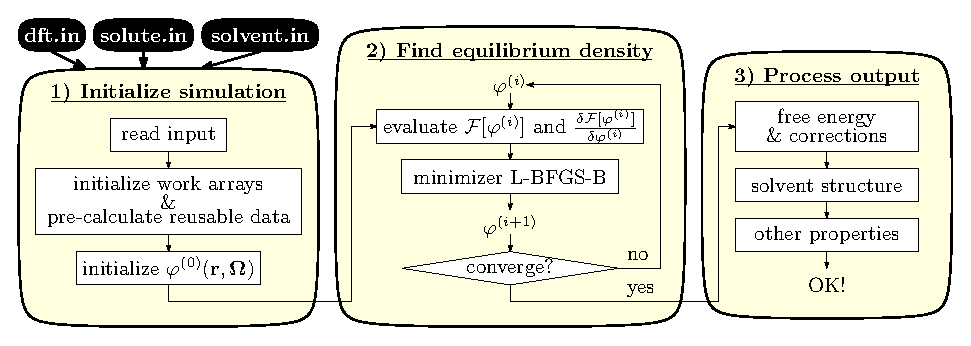
\includegraphics[width=0.5\paperwidth]{Front_Staff/mdft}\\
 \medskip{}
\par\end{center}

\begin{center}
\spacedlowsmallcaps{\mySubtitle}
\par\end{center}

\begin{center}
\spacedlowsmallcaps{\mysubtitle}
\par\end{center}

\vfill{}

\begin{center}
\bigskip{}
\par\end{center}

\begin{center}
\myTime @ \myLocation
\par\end{center}

\end{addmargin} 
\end{titlepage} 


\thispagestyle{empty}
\hfill

\vfill{}


\noindent\myName: \textit{\myTitle} \textit{\mytitle,} \mySubtitle,
\textcopyright\ \myTime

\begin{comment}
\bigskip{}
\noindent\spacedlowsmallcaps{Supervisors}: \\\myProf \\\myOtherProf \\\mySupervisor

\medskip{}
\noindent\spacedlowsmallcaps{Location}: \\\myLocation

\medskip{}
\noindent\spacedlowsmallcaps{Time Frame}: \\\myTime
\end{comment}



\cleardoublepage{}

\pdfbookmark[1]{Acknowledgments}{acknowledgments}

\begin{flushright}
\textsl{When you are studying any matter, or considering any philosophy,
ask yourself only, what are the facts and what is the truth that the
facts bear out.}\\
\textsl{ Never let yourself be diverted either by what you wish to
believe, or by what you think would have beneficent social effects
if it were believed.}\\
\textsl{ But look only, and solely, at what are the facts.}
\par\end{flushright}

\begin{flushright}
— Bertrand Russell 
\par\end{flushright}

\bigskip{}

\begingroup
\let\clearpage\relax
\let\cleardoublepage\relax 

\chapter*{Acknowledgements}

First of all, I would like to express my most respectful gratitude
to my thesis advisors, Daniel Borgis and Luc Belloni, who have developed
the main theories used in this thesis and whose great knowledge of
liquid theory as well as the genius way of thinking and explaining
have given me a solid guide for doing this research. I would also
like to thank them for their tireless work in correcting this manuscript.

I'm also grateful to Maximilien Levesque, the other main developer
of MDFT who joined the supervision of my thesis and the correction
of this manuscript. Thanks as well for sharing some results and data
that have proven useful to my research.

I wish to acknowledge all the great minds willing to evaluate and
give ideas about my work: Rodolphe Vuilleumier, Olivier Bernard, Bernard
Rousseau, Rosa Ramirez; thank you for agreeing to be part of the jury
of this thesis.

As a master student issued from pure chemistry speciality, a lack
of knowledge about Informatics brought to me a lot of difficulties.
I would like to express my sincere gratitude to my colleagues Pierre
Kestener, Matthieu Haefele, and Yacine Ould-Rouis for their huge aid
in Informatics and very useful advices during this thesis.

This thesis was produced at\textit{ Maison de la Simulation, CEA Saclay},
financially supported by the schola\textcolor{black}{rship IDEX-CEA.
I }acknowledge all the organizations and staff that gave me the chance
to have this three-year experience.

I am also grateful to Thomas Wiggins for help in correcting the huge
amount of grammar faults in this manuscript.

Looking back through all those years of schooling, I'm deeply indebted
to my tutors during my bachelor and master, respectively Mr. Hongwei
Tan and Mrs. Michelle Gupta, whose clear logic and warm encouragement
gave me all that I needed to be in love with theoretical chemistry.

And I should also thank my friends Yiting Cui, Qirong Zhu, Yu Wu and
Bo Gao for taking care of me at the very end of the thesis when I
was seriously ill.

Finally I would like to thank my father, who made the right decision
to send me here in France and support me in every aspect.

\endgroup


\cleardoublepage{}

\pagestyle{scrheadings}

%*************************
% Table of Contents
%*************************
%\phantomsection
\refstepcounter{dummy}
\pdfbookmark[1]{\contentsname}{tableofcontents} 
\setcounter{tocdepth}{2} % <-- 2 includes up to subsections in the ToC 
\setcounter{secnumdepth}{3} % <-- 3 section numbers up to subsubsections 
\manualmark 
\markboth{\spacedlowsmallcaps{\contentsname}}{\spacedlowsmallcaps{\contentsname}} 
\tableofcontents  
\automark[section]{chapter} 
\renewcommand{\chaptermark}[1]{\markboth{\spacedlowsmallcaps{#1}}{\spacedlowsmallcaps{#1}}} \renewcommand{\sectionmark}[1]{\markright{\thesection\enspace\spacedlowsmallcaps{#1}}} 

\clearpage{}

\begingroup
\let\clearpage\relax
\let\cleardoublepage\relax

%*************************
% List of Figures     
%*************************
%\phantomsection
\refstepcounter{dummy}
%\addcontentsline{toc}{chapter}{\listfigurename}
\pdfbookmark[1]{\listfigurename}{lof}
\listoffigures

\vspace{8ex}

%*************************
% List of Tables
%*************************
%\phantomsection
\refstepcounter{dummy}
%\addcontentsline{toc}{chapter}{\listtablename}
\pdfbookmark[1]{\listtablename}{lot}
\listoftables

\vspace{8ex}

%*************************
% Notations
%*************************
%\phantomsection
\refstepcounter{dummy}
\pdfbookmark[1]{Notations}{notations}
\markboth{\spacedlowsmallcaps{Notations}}{\spacedlowsmallcaps{Notations}}
\chapter*{Notations} 

\hspace{-0.5em}%
\begin{tabular}{>{\raggedright}p{3.3em}l}
$\mathcal{F}[\rho]$ & Solvation free energy functional {[}$\mathrm{kJ\cdot mol^{-1}}${]}
-\tabularnewline
\end{tabular}

\hspace{-1.5em}%
\begin{tabular}{>{\raggedright}p{3.3em}l}
$\rho(\mathbf{r},\mathbf{\Omega})$ & Density of solvent {[}$\textrm{\AA}^{-3}${]}-\tabularnewline
\end{tabular}

\hspace{-1.5em}%
\begin{tabular}{>{\raggedright}p{3.3em}l}
$\mathcal{F}_{\mathrm{id}}[\rho]$ & Ideal free energy functional {[}$\mathrm{kJ\cdot mol^{-1}}${]} -\tabularnewline
\end{tabular}

\hspace{-1.5em}%
\begin{tabular}{>{\raggedright}p{3.3em}l}
$\mathcal{F}_{\mathrm{ext}}[\rho]$ & External free energy functional {[}$\mathrm{kJ\cdot mol^{-1}}${]}
-\tabularnewline
\end{tabular}

\hspace{-1.5em}%
\begin{tabular}{>{\raggedright}p{3.3em}l}
$\mathcal{F}_{\mathrm{exc}}[\rho]$ & Excess free energy functional {[}$\mathrm{kJ\cdot mol^{-1}}${]}- \tabularnewline
\end{tabular}

\hspace{-1.5em}%
\begin{tabular}{>{\raggedright}p{3.3em}l}
$\gamma(\mathbf{r},\mathbf{\Omega})$ & Gradient of excess free energy functional, {[}$\mathrm{}${]}-\tabularnewline
\end{tabular}

\hspace{-1.5em}%
\begin{tabular}{>{\raggedright}p{3.3em}l}
$q_{e}$ & Elementary charge, $q_{e}=1.602176565\cdot10^{-19}\,\mathrm{[C]}$\tabularnewline
\end{tabular}

\hspace{-1.5em}%
\begin{tabular}{>{\raggedright}p{3.3em}l}
$\varepsilon_{0}$ & Vacuum permittivity, $\varepsilon_{0}=8.854187817\cdot10^{-12}\,\mathrm{[C^{2}\cdot J^{-1}\cdot m^{-1}]}$\tabularnewline
\end{tabular}

\hspace{-1.5em}%
\begin{tabular}{>{\raggedright}p{3.3em}l}
$N_{\mathrm{A}}$ & Avogadro constant, $N_{\mathrm{A}}=6.02214129\cdot10^{23}\,\mathrm{[mol^{-1}]}$.\tabularnewline
\end{tabular}

\hspace{-1.5em}%
\begin{tabular}{>{\raggedright}p{3.3em}>{\raggedright}p{0.87\columnwidth}}
$f_{Q}$ & $f_{Q}=q_{e}^{2}10^{-3}N_{\mathrm{A}}/(4\pi\varepsilon_{0}10^{-10})$,
electrostatic potential unit so that $f_{Q}\cdot q^{2}/r$ is in {[}$\mathrm{kJ\cdot mol^{-1}}${]},
where $q$ is the number charge without unity, $r$ in {[}$\textrm{\AA}${]}.\tabularnewline
\end{tabular}

\hspace{-1.5em}%
\begin{tabular}{>{\raggedright}p{3.3em}l}
$K_{\mathrm{B}}$ & Boltzmann constant, $K_{\mathrm{B}}=1.3806488\cdot10^{-23}\,[\mathrm{J\cdot K^{-1}}]$\tabularnewline
\end{tabular}

\hspace{-1.5em}%
\begin{tabular}{>{\raggedright}p{3.3em}>{\raggedright}p{0.87\columnwidth}}
$\rho_{0}$ & Bulk solvent angular density, $n_{0}=\int\mathrm{d}\mathbf{\Omega}\rho_{\text{0}}=8\pi^{2}\rho_{0}$
is the bulk solvent number density, both of unity {[}$\mathrm{\textrm{\AA}^{-3}}${]}-\tabularnewline
\end{tabular}

\hspace{-1.5em}%
\begin{tabular}{>{\raggedright}p{3.3em}l}
$\beta$ & $\beta=\left(K_{\mathrm{B}}T\right)^{-1}$, reciprocal of the thermodynamic
temperature {[}$\mathrm{mol\cdot kJ^{-1}}${]}\tabularnewline
\end{tabular}

\hspace{-1.5em}%
\begin{tabular}{>{\raggedright}p{3.3em}l}
$ $ & \tabularnewline
\end{tabular}

\vspace{8ex}

%*************************
% Acronyms
%*************************
%\phantomsection
\refstepcounter{dummy}
\pdfbookmark[1]{Acronyms}{acronyms}
\markboth{\spacedlowsmallcaps{Acronyms}}{\spacedlowsmallcaps{Acronyms}}
\chapter*{Acronyms}
\begin{acronym}[UML]
  \acro{DCF}{direct correlation function}
  \acro{DFT}{discret Fourier transform, also refers to density functional theory}
  \acro{FE}{function evaluation}
  \acro{FFT}{fast Fourier transform}
  \acro{FGSHT}{fast generalized spherical harmonic transform}
  \acro{GSH}{generalized spherical harmonic}
  \acro{GSHT}{generalized spherical harmonic transform}
  \acro{HNC}{hypernetted-chain (approximation)}
  \acro{HRF}{homogeneous reference fluid (approximation)}
  \acro{IET}{integral equation theory}
  \acro{MC}{Monte Carlo}
  \acro{MD}{molecular dynamics}
  \acro{MDFT}{molecular density functional theory}
  \acro{MOZ}{molecular Ornstein-Zernike (equation)}
  \acro{OZ}{Ornstein-Zernike (equation)}
  \acro{PCF}{pair correlation function}
  \acro{PDF}{pair distribution function}
  \acro{QM}{quantum mechanics} 
\end{acronym}              

\endgroup

\cleardoublepage{}


\cleardoublepage{}

\pagenumbering{arabic}


\chapter{Introduction\label{chpt:introduction}}

This thesis details the development of an original numerical toolkit for
physical chemists and structural biologists, based on the molecular
density functional theory (\acs{MDFT}), which makes it possible to
predict the solvation properties of arbitrary molecular objects in arbitrary molecular solvents
(mainly water) efficiently and with microscopic accuracy. This introduction will help to understand the objective
of this thesis, it explains why people are interested in the nature
of solvation, and where we are in terms of the computing trends in solvation
simulations.


\section{Simulation of solvent effects}

Solvation is a fundamental phenomenon in chemistry. The chemical behavior
of numerous systems strongly depends on the nature of solvency, including popular issues like metal-organic reacting centers
\citep{Mn-oxo,PCET}, or pharmaceutical etudes \citep{drug_1_Perlovich,drug_2_Perlovich,drug_3}.
The solvation properties required by etudes %Etude? I only know this in terms of music. Does it have scientific applications?
are highly variable, such
as the Gibbs free energy of solvation, solubility, partition coefficient,
saturated vapor pressure, pH value, the 3D solvation structure,
etc. Overall, the interest in these solvation properties reaches into
many domains such as chemistry, biochemistry, pharmaceuticals, medicine, and
environmental and agrochemical industries. Unlike the well-studied
quantum mechanics (\acs{QM}) for chemical interaction and macroscopic
finite element model for physical processes, the theories of solvation
are quite variable and still under development, owing to the ambiguous
compromise between accuracy and computing cost. In a word,
the studies in this domain are quite vibrant.

\begin{figure}[h]
\centering{}\textcolor{red}{}%
\begin{minipage}[t]{1\textwidth}%
\begin{center}
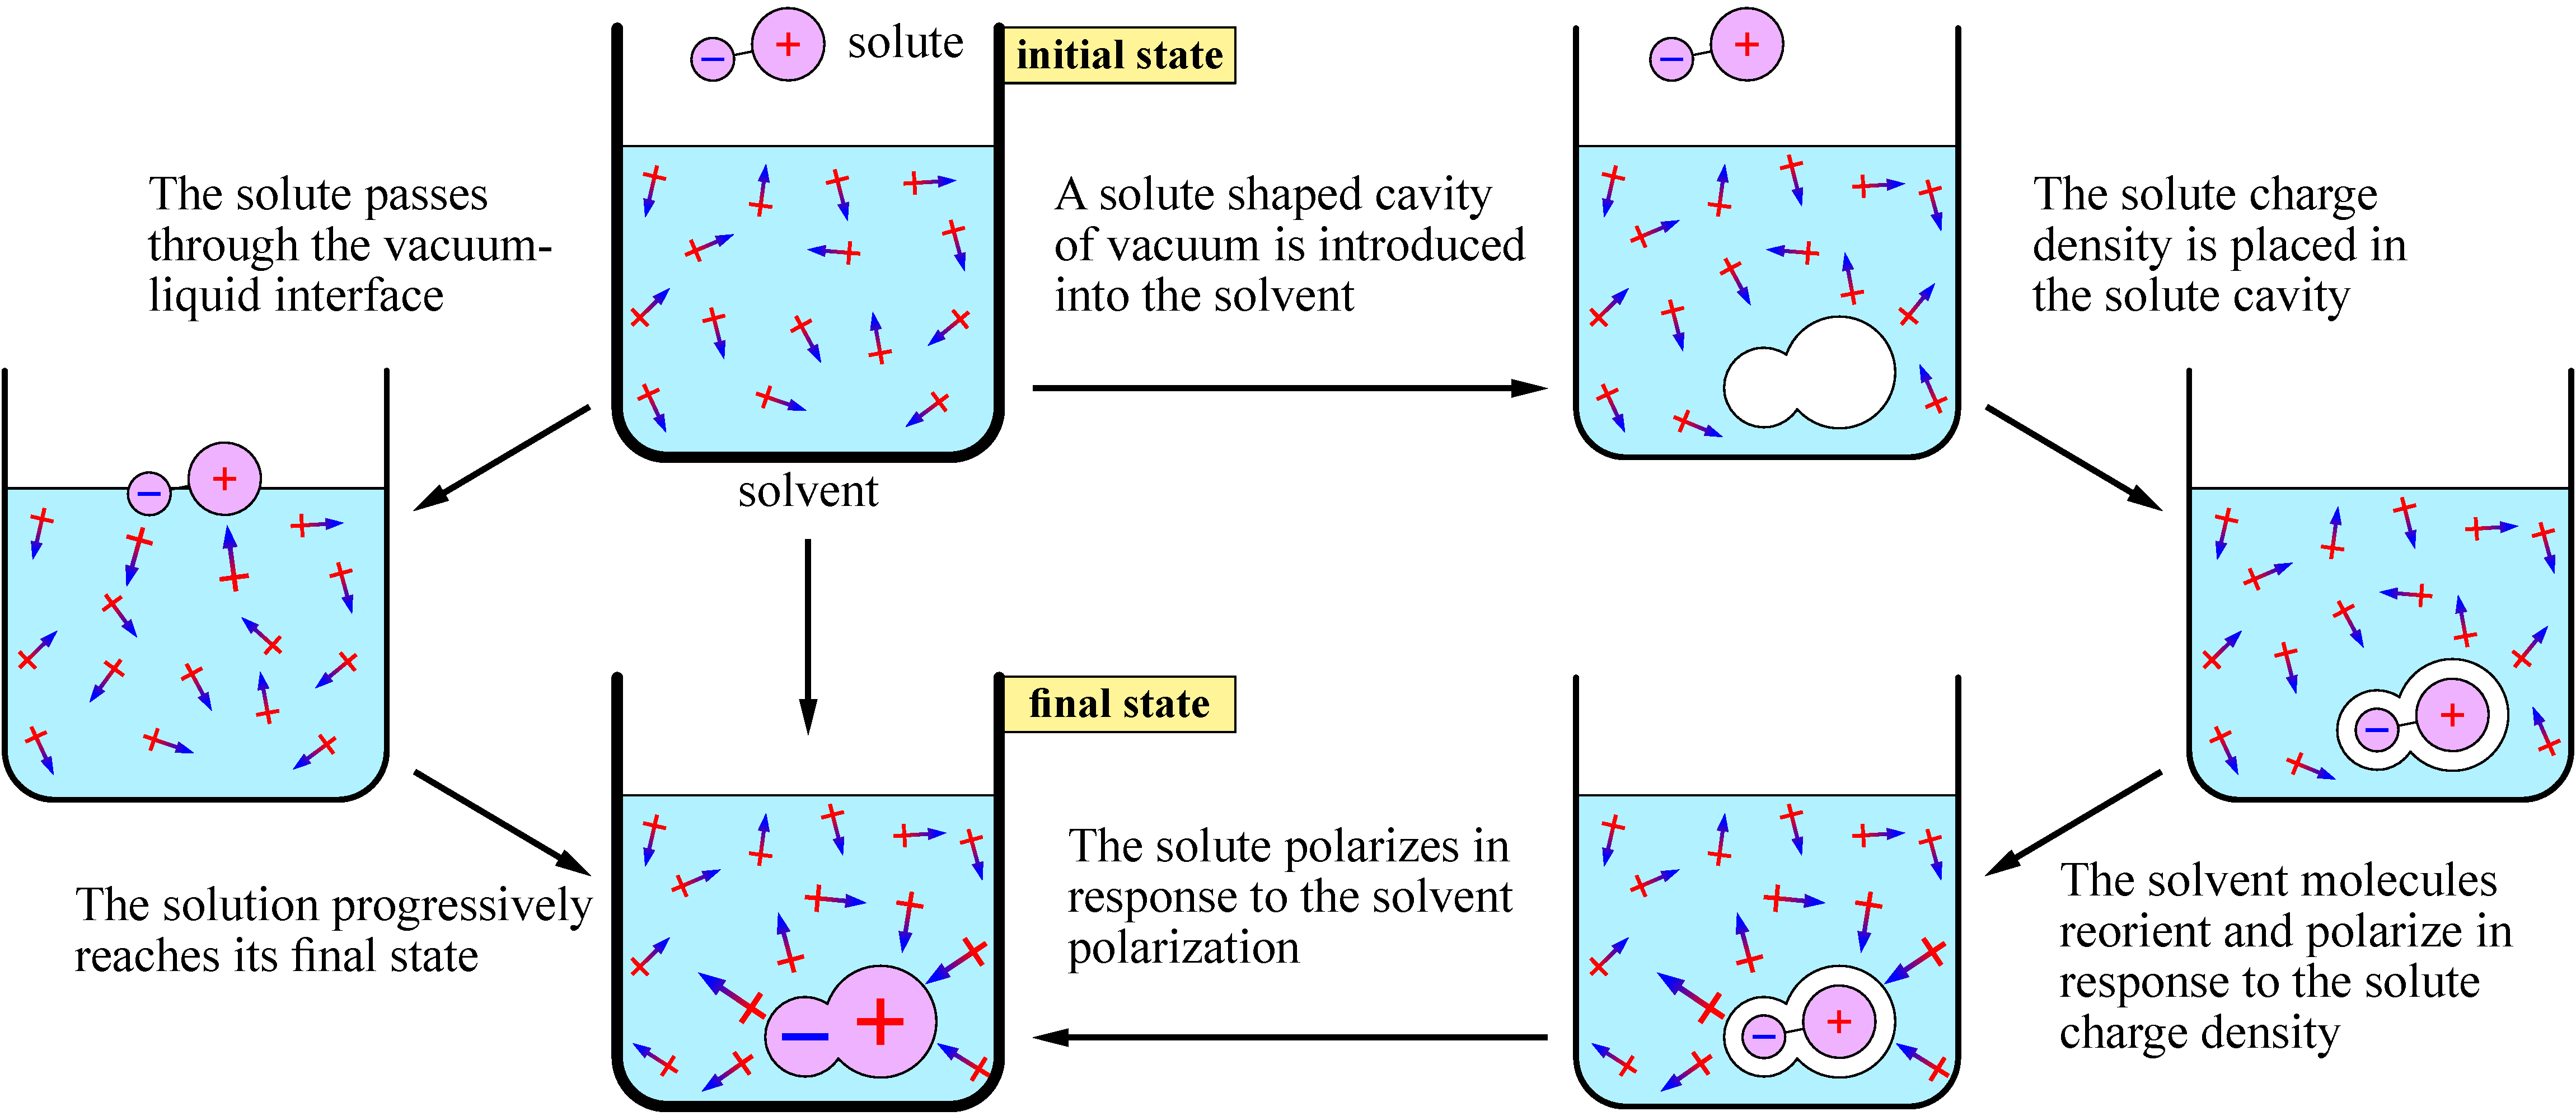
\includegraphics[width=1\columnwidth]{_figure/solvation}\caption[The solvation process]{The solvation process.\label{fig:Process-of-solvation} A thermodynamic
system, whose properties only depend on the initial and final states,
can go through different paths. The physical process of solvation
(left path) takes the solute from vacuum into bulk solvent, progressively
passing through the vacuum-liquid interface. Theoretically, the solvation
energy is defined as the energy consumed in such a process. In theoretical
studies, the process can be decomposed to some artificial unphysical
process (right path), involving the growth of an uncharged solute-sized
cavity within the bulk solvent, the transfer of the solute charge
distribution from vacuum into cavity, and the interaction between
the solute and solvent.}

\par\end{center}%
\end{minipage}
\end{figure}


To change a phenomenon to a model, we must first understand its process.
Solvation is defined as the process of moving a molecule from the
gas phase (or vacuum) to a condensed phase (figure \ref{fig:Process-of-solvation}),
which builds a stabilizing interaction with the solute (or solute
moiety like protein residues, interfaces, etc.) \citep{iupac}. Such
interactions are mostly classical, involving electrostatic
and van der Waals forces, with additional more specific chemical effects
such as hydrogen bond formation, and quantic effects for some small
solvents whose vibrational or rotational energy states are at the same
magnitude as $k_{\mathrm{B}}T$, etc. \citep{Gray-Gubbins}.

As not all kinds of interactions are important in applications, according
to the usage, different models and methods have been developed.

For most of the 20th century \citep{Cramer_1999}, the study of
solvation effects has been dominated by continuum (implicit) models,
which depend upon the dielectric constants and are not costly
in terms of computation resources. They provide an accurate way to treat the
strong, long-range electrostatic interactions which dominate many
solvation phenomena, but lack detailed information on the first
solvation shell. The latter, which mainly includes the cavity formation
energy and solute-solvent van der Waals interactions, is often rudely
treated by introducing an artificial form of cavity that links to the
form of solute. The methods for testing electrostatic interactions include
generalized Born model, or for better estimates via Poisson-Boltzmann
calculations. They are widely integrated within \acs{QM} simulations
of the solvent, by add extra solvation terms onto the Fock or Kohn-Sham
operator \citep{Jensen,scrf,Tomasi_1994_implicit_model}. However,
the improper treatment of the first-shell, where the microscopic interactions
are primarily located, often introduce sometimes huge error in free
energy evaluation, especially for polar solvents (like water), despite
the accuracy that the \acs{QM} calculation alone can achieve. Therefore,
classical molecular simulations, which describing the individual solvent
molecules (explicit), particularly the molecular dynamics (\acs{MD})
and Monte Carlo method (\acs{MC}), became the alternative solution
during the last few decades. They generate trajectories and configurations,
then estimate free energy changes by statistical mechanic technics,
such as free energy perturbation (FEP) theory or thermodynamic integration
(TI) \citep{Jorgensen_1995_MC}. These calculation is very demanding
on computing cost, due to the requirement of many (hundreds or thousands
of) solvent molecules to form a realistic model.

Recently, a third domain of theory to describe solvent, based on the
statistical mechanics of fluid, is growing rapidly. It is generally
called liquid theory, involves mainly the integral equation theory
(\acs{IET}), and the classical density functional theory for liquids.
These approaches are cope to give the molecular nature of the first-shell,
but without calculate all the instantaneous micro-states with respect
to time, which can be integrated over positions and momentums theoretically.
Therefore, they are of magnitudes faster than those simulations by
micro-states.

The integral equation theory (\acs{IET}) is about solving the Ornstein-Zernike
(\acs{OZ}) equation with a specific closure equation \citep{Hensen-McDonald,Gray-Gubbins}.
It was firstly limited to so called ``simple liquid'' - a system
of spherical particles. A part, Chandler and Andersen in 1971 \citep{Chandler_1972_RISM}
developed the reference interaction site model (\acs{RISM}), which
discretizes the distribution and correlation functions into a site-site
set of functions, and solve the \acs{OZ} equation in matrix \citep{hirata_molecular_2004}.
Another part, Blum \citep{Blum_I,Blum_II}, Fries and Patey \citep{Fries_Patey_1985}
extend the \acs{OZ} equation to molecular case, where the distribution
and correlation functions depend on both position and orientation.
In their theory, the orientation part of \acs{OZ} equation is simplified
by expending the distribution and correlation functions on Wigner
generalized spherical harmonics.

The classical density functional theory approach deal with inhomogeneous
liquids, which uses the same variation principle and minimization
strategy \citep{mermin_thermal_1965,Evans_1979,Hansen_1987} as electronic
density functional theory \acs{DFT} that treats electric interactions
and has a great success in computational chemistry. It gives the Helmholtz
free energy and the equilibrium solvent density, by minimizing the
free energy functional of the solvent density in the presence of a
given external potential. Borgis and collaborators \textcolor{red}{{[}too
many ref{]}} have recently generalized it into molecular case, named
molecular density functional theory (\acs{MDFT}), where the solvent
density depends on both position and orientation, $\rho(\mathbf{r},\mathbf{\Omega})$.
The main theoretical difficulty lies in the definition of well-funded
and reliable functionals of the excess free energy $\mathcal{F}_{\mathrm{exc}}\left[\rho\right]$,
according to the geometric complexity of the solvent molecule. Some
recent researches have shown that it is cope with linear solvents
like acetonitrile, but still have little non-satisfaction with the
most complex solvent, i. e. water. \acs{MDFT} can be proved to be
mathematically equivalent to the two-component molecular \acs{IET}.

The majority of work of all these theories have been focused on water,
since it is one of the most difficult systems to model due to its
molecular geometry, ineligible multi-body interaction, quantum effect,
hydrogen bond, etc. The importance of including instantaneous polarization
in potential functions is also an issue \citep{polarisable_1,polarisable_2}.
However, since polarizable force fields are not yet in common use,
the simulations by micro-states and the liquid theory which feed on
force field also have their own limit, compared to the continuum model
which can be polarizable. The advantages and disadvantages of each
branch of theory are listed in table \ref{tab:Theories-of-solvation}.

\begin{table}[h]
\begin{centering}
\begin{tabular}{ccccc}
\toprule 
\tableheadline{Theory} & \tableheadline{Speed} & \tableheadline{Long-Range} & \tableheadline{First-Shell} & \tableheadline{Polarizable Solvent}\tabularnewline
\midrule
Continuum model & fast & yes & no & fully\tabularnewline
Simulation by time & costly & yes & yes & partially, very costly\tabularnewline
Liquid theory & fast & yes & yes & partially\tabularnewline
\bottomrule
\end{tabular}
\par\end{centering}

\caption{Theories of solvation simulation\label{tab:Theories-of-solvation}}
\end{table}


This thesis consists in the development of the \acs{MDFT}, focusing
on the generalization and algorithmic acceleration of the excess free
energy functional $\mathcal{F}_{\mathrm{exc}}$ evaluation under homogenous
reference fluid (\acs{HRF}) approximation, which will be discussed
in detail in later chapters. 


\section{Scope of this thesis}

Chapter I reviews a selection of models and methods to the solvent
effect. It includes the mainly used continuum model, the basic of
liquid theory, as well as its two frontier research domains, \acs{IET}
and \acs{MDFT}. The code structure of \acs{MDFT}, which all the
development in this thesis is based on, is also presented. There is
also a brief introduction to \acs{MD} and \acs{MC}, as well as the
generation of direct correlation function (\acs{DCF}) used in this
thesis by such methods. 

Chapter II presents all the theory developed and newly used in this
thesis. In this thesis, two algorithms of excess energy functional
evaluation are proposed, one is extension of the previous algorithm,
other is a new algorithm, that combines the molecular \acs{OZ} equation
treatment of angular part with MDFT. The output solvation properties
is mainly the two: free energy, and solvent structure.

Chapter III takes note of all the implementation result, that divided
into two aspects, the ``accuracy'', which involves comparisons between
algorithms, and with \acs{IET} and \acs{MD} results; and the ``efficiency'',
which evaluate the computing cost of the code, both in sequential
and parallelized version.

Chapter VI gives some application to ions and molecules.



\ctparttext{\textcolor{red}{(Chapter introduction is to clear the motivation
and relation between sections.)}\\
\medskip{}
This chapter is a summary of all the previous work that this thesis
is based on.\\
\medskip{}
In section \ref{chpt:models}, we begin by introducing the models
used in our study, as well as some other examples of different scale
or description by way of comparison to illustrate why we chose our models. \\
\medskip{}
Once the model is chosen, all the theories become mathematical problems.
Section \ref{chpt:statistical-mechanics} reviews some basic concepts
of statistical mechanics for liquids (liquid theory), which present
the deduction of formalisms from the model of the system, without
introducing any artificial terms. The following two sections, section
\ref{chpt:iem} and \ref{chpt:mdft} give two frontier domains of
the liquid theory that this thesis works upon: the integral equation theory (\acs{IET}), and
the molecular density functional theory (\acs{MDFT}). A clear mathematical equivalence between these two theories
is presented in section \ref{chpt:mdft}, which gave
us the idea to use the expansion techniques in \acs{IET} to serve \acs{MDFT}.\\
\medskip{}
Finally, a brief introduction of the simulations deployed here is made in section \ref{chpt:reference-method}. Depending on micro configuration, this includes molecular dynamics (\acs{MD}) and
Monte Carlo (\acs{MC}) simulation methods.
This is done to explain how the direct correlation functions (\acs{DCF})
portrayed in this thesis are obtained.}


\part{State of the Art: Solvation, Models and Methods}%Unfamiliar with word 'solvation'; is this a technical term?

\cleardoublepage{}

\appendix

\part{Appendix}


\chapter{Basic Concepts about Computing Performance\label{chpt:computing-performance}}

In addition to the theory, the performance of the code being developed is
also an important aspect of this thesis. It is essential to
have a fast and accurate method. To evaluate a code in a strict and
systematic way, some basic concepts of computing performance are listed
here. 


\section{Algorithm complexity}

Algorithm complexity is a crucial criteria for sequential code.
A definition is given below.

Let $f$ and $g$ be two real (or even complex) functions defined
over the natural numbers $\mathbb{N}$. We write
\begin{equation}
f=O(g)
\end{equation}
if there is a constant $c>0$ such that from certain number $n>n_{0}$
we always have $\left|f(n)\right|\leq c\left|g(n)\right|.$ The $O$
is also named as the big-O notation \citep{Complexity}, or order
of growth. Figure \ref{fig:order-of-growth} shows the growth tendency
of some frequent functions; from this we can conclude the following: 
\begin{equation}
O(1)>O(\log_{2}n)>O(n)>O(n\log_{2}n)>O(n^{2})>O(2^{n})>O(n!)
\end{equation}


\begin{figure}[h]
\begin{centering}
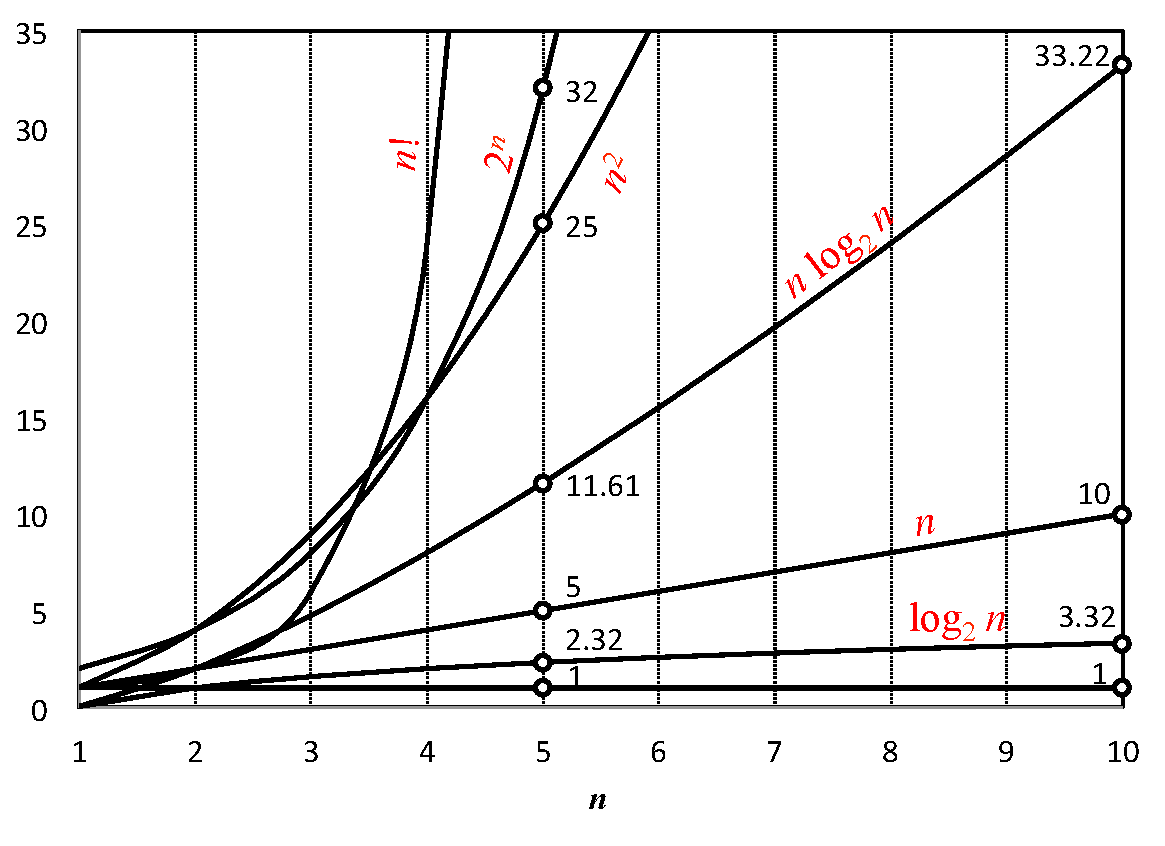
\includegraphics[width=0.65\textwidth]{_figure/orders-of-growth}
\par\end{centering}

\caption{Function growth\label{fig:order-of-growth}}
\end{figure}


In this thesis, the big-O notation is used to measure algorithm complexity.
Other notations can also be used for the same purpose, such as: 
\begin{itemize}
\item $f=o(g)$ if $f(n)/g(n)\rightarrow0$, $n\rightarrow\infty$
\item The inverse of big-O notation $f=\Omega(g)$ if $g=O(f)$
\item The notation $f=\Theta(g)$ means that both $f=O(g)$ and $g=O(f)$
hold, and we can also say they are of the same order.
\end{itemize}
In a code, we always search algorithms with a lower algorithm complexity.
Ideally, the implementation of code matches the model and has the
same growth tendency as its complexity, but in terms of practicality,
overheads and memory delay can also limit the performance. \textcolor{red}{(part
to be modified to adapt implementation results)}


\section{Roofline model and memory delay}

The simplest model aiming to distinguish whether a piece of code is
limited by the computing power (CPU) or the memory bandwidth (RAM
to Caches) is the roofline model \citep{Williams_2009_roofline} for
single loop:
\begin{equation}
P=\min\left(P_{\max},\,I\cdot b_{\mathrm{S}}\right)\label{eq:roofline}
\end{equation}
where

\begin{tabular}{l>{\raggedright}p{0.9\textwidth}}
$P$ & is the applicable peak performance of a loop, assuming that data comes
from the level 1 cache, of unity $\mathrm{GFlop/s}$. \tabularnewline
$I$ & is the computational intensity (“work” per byte transferred) over
the slowest data path utilized, of unity $\mathrm{Flop/Byte}$. \tabularnewline
$b_{\mathrm{S}}$ & is the applicable peak bandwidth of the slowest data path utilized,
of unity $\mathrm{GByte/s}$.\tabularnewline
 & \tabularnewline
\end{tabular}

As shown in figure \ref{fig:The-roofline-model}, the overall performance
is limited by both the peak performance and the memory bandwidth.
The computational intensity $I$ depends on the code, while the other
two terms in eq. (\ref{eq:roofline}) depend on hardware. The optimal
use of resources occurs at the intersection point.

\begin{figure}[h]
\begin{centering}
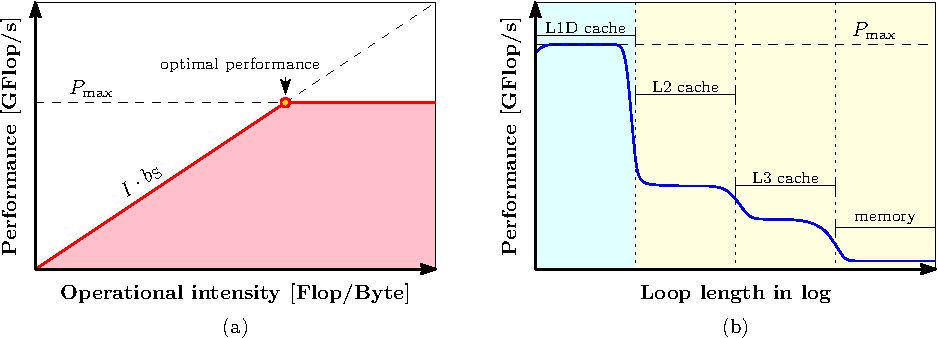
\includegraphics[width=1\columnwidth]{_figure/roofline}
\par\end{centering}

\caption [The roofline model and performance pattern]{The roofline model and performance pattern. (a) The roofline model.
(b) Performance pattern of a simple loop with respect to the loop
length in logarithm. The blue part is limited by operation execution,
and the yellow part by memory bottleneck. \label{fig:The-roofline-model}}
\end{figure}


The roofline model can give an idea of whether the diminuition of algorithm
complexity is the most important optimization strategy, because it
only counts the number of operations. In most of cases, avoiding
slow data paths is the key to performance optimization.

As shown in figure \ref{fig:Memory}, the memory hardware has hierarchical
architectures. The fastest ones are the registers included in the
microprocessor, which are used for temporary storage of data, instructions
and addresses required by the arithmetic logic unit (ALU) and the
control unit (CU) in CPU during execution of a program. The lowest
is normally the input/output (I/O) process. The reading strategy of
data (contiguous or not), as well as the size and initialized location of arrays,
both play pivotal roles in the overall computing performance. 

\begin{figure}[h]
\begin{centering}
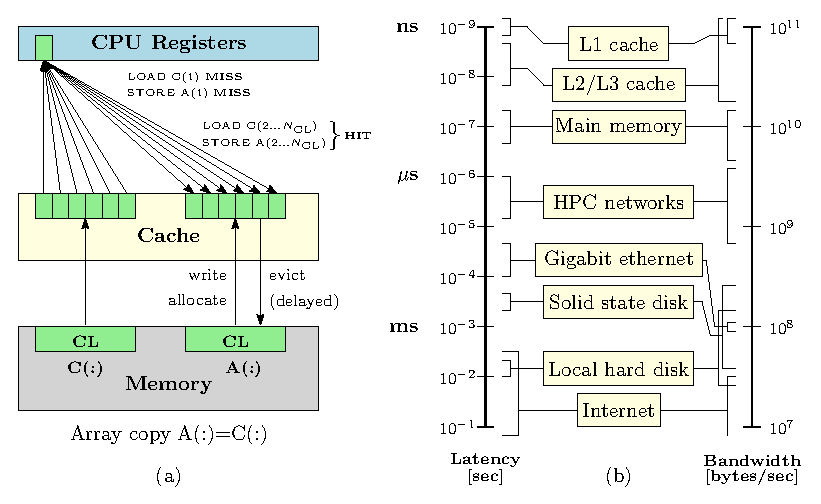
\includegraphics{_figure/memory}
\par\end{centering}

\caption [Memory usage in hardware level]{Memory usage in hardware level \citep{LRZ-cours}. (a) An example
of array copy A(:)=C(:). Caches are organized in cache lines (CL);
only complete cache lines are transferred between memory hierarchy
levels (except registers). HIT/MISS: Load or store instruction does/doesn't
find the data in a cache level. (b) Computing latency and memory bandwidth
vary by magnitude, from the fastest cache transfers to the lowest
processes.\label{fig:Memory}}
\end{figure}



\section{Scalability of parallelized code}

For parallelized code, scalability is the key issue. Highly scalable
codes can take advantage of numerous nodes of HPC centers, so that
single core performance no longer matters. 

The speed-up is defined as:
\begin{equation}
S(N)=\dfrac{t(1)}{t(N)}
\end{equation}


And the relative efficiency is:
\begin{equation}
E(N)=\dfrac{S(N)}{N}=\dfrac{t(1)}{Nt(N)}
\end{equation}


$S(N)\sim N$ or $E(N)\sim100\%$ means the application scales. 
By contrast, $S(N)<N/2$ or $E(N)<50\%$ means the application does
not scale. 

Amdahl's Law gives the theoretical speedup in latency of the execution
of a task at fixed workload:
\begin{equation}
S(N)=\dfrac{1}{\alpha_{\mathrm{s}}+\alpha_{\mathrm{p}}/N}
\end{equation}
where $\alpha_{\mathrm{s}}$ is the serial fraction and $\alpha_{\mathrm{p}}$
the parallel fraction of the source code. Therefore the overall computing
speed is limited by the unscalable part:
\begin{equation}
\lim_{N\rightarrow\infty}S(N)=\frac{1}{\alpha_{\mathrm{s}}}
\end{equation}
making it the focus we wish to reduce.


\section{Profiling and tracing toolkits}

There are several types of software and toolkits for performance evaluation.
They are of two categories: profiling and tracing. A trace is a collection
of events or timestamps. A profile is a collection of timings. Profiling
tools are usually more simple and rapid, but for subroutines that are called
a large number of times, the overhead in time measurement is negligible. 

The tool used in this thesis is mainly VTune, where application execution
is interrupted every $\sim100\,\mathrm{\mu s}$ and information is
stored (call stack, hardware counters, etc.). The execution time overhead
is small. \textcolor{red}{(To be detailed.)}


\cleardoublepage{}

%*************************
% Bibliography 
%*************************
% work-around to have small caps also here in the headline
\manualmark \markboth{\spacedlowsmallcaps{\bibname}}{\spacedlowsmallcaps{\bibname}}
%\phantomsection
\refstepcounter{dummy}
\addtocontents{toc}{\protect\vspace{\beforebibskip}}
% to have the bib a bit away from the rest in the toc
\addcontentsline{toc}{chapter}{\tocEntry{\bibname}}

\label{app:bibliography}

\printbibliography

\end{document}
